\setcounter{chapter}{ 14 }
\chapter{\textbf{Nicklepan, City Station A, Part 1} }






\textit{Notes:} Suko

\textit{Date:} January 29th, 2013



Bad things happened in Nicklepan.  Mom, Dad, don't touch it!  It's eeeevillll.



Update 1/31/13 ~5:30pm:  Now with pretty pictures!  See the end of the document.  Thanks Nate!  That should help clarify the ``who is where'' planning.



\noindent\hrulefill





 {\LARGE City Station A } 



The train pulls into the station.  Jaya dramatically rips off the bandage over her new tattoo and readies her gun.  She and Lackovich jostle slightly for position at one door, while Hayley stands at the other door.  Oliver stands slightly behind her, rifle ready, and Jonah behind them and to one side.  As the train slows and the doors are about to open, Jonah tells Hayley to get out of the doorway.  She turns around to looks at him in confusion as the doors open.  She doesn't duck, but instead just steps slightly to one side, as if someone was going to walk past her through the door.



They are immediately met by a wave of heat and humidity, far more than they have felt anywhere in the Directorate.



The station platform is wide open, perhaps the most open platform any of us have seen.  It extends for about 15' and is surrounded by a chain link fence.   To one side there is a gate in the fence that leads to a series of switchbacks that eventually lead to the other side of the fence.  The station is above ground and there are pillars holding up a roof supplying shade.  On the other side of the fence is a road, and on the other side of the road, there are shanty-town-like buildings. The buildings are short 1-2 story buildings, with corrugated metal sides.  There is an identical platform and fence setup on the other side of the tracks.



Jaya asks Lackovich, ``So does this compare to your previous experience?''

``You do realize I've never been here before, right?''

``Well, still, how does it compare?''

``I'd say it's strange.''



{[}\textit{Challenge: The Iron Road.  }\textit{4 Threat Tokens enter the pool}{]}



Jaya steps off of the train and Hayley immediately copies her.  Jaya uses the new binoculars to scan the area. {[}\textit{Challenge: Notice Movement 1.  Overcome}{]}.  Oliver hooks up the antenna and listens for sounds of activity.  {[}\textit{Challenge: Notice People 2.  Overcome}{]}.  Hayley heads straight for the gate and discovers that it is locked.  She points this out to Jaya, who comes over and tells her to open it.  When Hayley asks how, Jaya says she should shoot the lock off with her rifle.  Jaya does warn her to be careful not to shoot anyone else nearby while she does it. {[}\textit{Challenge: Break the lock 1.  Overcome}{]}



Hayley shoots the lock off and yelps in surprise at the substantial kick of the much more powerful rifle.  At the sound of unexpected gunfire, Jonah drops and dives for cover by the fence.  Oliver drops the antenna, crouches, raises his rifle and starts scanning the area for shooters. 



Oliver yells, ``What the fuck was that?''

``We opened a door!'' yells back Jaya and then picks up the binoculars and scans the buildings nearby, thinking to herself that she should see something now if anyone is around.



Hayley looks around and sees Jonah on the ground.  Alarmed, she runs over to him. ``Are you okay?''

``Yes.  What were you doing?''

``Opening a lock.''

``With a rifle?!''.  Jonah looks incredulous.

``Yes.''

``Why?''

``Because that's how I was told to open it.'' 

``Well next time warn everyone before you shoot a rifle!''

``Okay.''  Hayley looks over at Oliver and rubs her shoulder with a grimace.  ``Is it supposed to hurt that much?''

``Yeah it has a pretty strong kick.  You really need to seat the gun firmly into your shoulder.  Otherwise it could knock you over.''



Despite the ruckus, it seems like no one has noticed their arrival -- and in fact that there is no one around at all.  Oliver and Jonah express their disapproval of the frivolous and potentially dangerous gunfire, but Jaya says that there is no one around, so it was fine.  Oliver reluctantly concedes that he also hasn't heard anything living in the area.  The area appears to be completed deserted and Jonah suggests in a toneless way that there may have been a plague. 



They head through the gate and to the road.  To the right there is a building which Lackovich says is probably a ticket station.  ``Let's see if the tickets are any cheaper here!'' jokes Jaya and gets a look from Lackovich.



They search the ticket station.  It is empty and has been for a while.  There are scattered boxes but most are opened and empty.  Jaya has Hayley climb onto the roof to get a better view of the surrounding area.



While Hayley is looking around, Oliver asks Lackovich if she knows if the people in Nicklepan were nervous about anything when she knew them.  ``I don't know'' she replies.  ``I haven't seen them in over a year.  They weren't nervous then.''



Hayley reports that there are mostly \hl{1-story small buildings}\footnote{\textbf{q.google }Nate noted that the buildings were unusually short from the POV of the Directorate. \textsubscript{01/31/13 1:00pm}}\footnote{$\rightarrow$\textbf{Suko T }I also got the impression that they are more flimsy in construction than we are used to seeing, especially for such a large and permanent-looking habitation (certainly anything near a train station anyway).  Directorate ruins may be ruins but at least they are made with cement and brick :) \textsubscript{01/31/13 2:02pm}}\footnote{$\rightarrow$\textbf{Nathaniel Ford }There is plenty of cement, but there is also a lot more corrugated steel and fabricated planking. And as noted the buildings are shorter. \textsubscript{01/31/13 3:39pm}} where they are, and slightly taller buildings across the tracks.  Behind the short buildings there is a funny looking area where there are no buildings, that is brown and flat.  It doesn't look like fire, at least not any fire damage she has seen.  The train tracks head out of an area where the ground slopes up slightly (the direction they presumably came from), and head toward an area in the distance where she can see much taller buildings.



Hayley jumps down from the roof and Jaya thinks about what they should do.  Oliver and Jonah suggest that there are more likely to be people and useful information in the area with the large buildings so Jaya decides that they will head into the downtown.  Rook is not reachable by radio so Jaya orders the group to split up and do a short-range area search for about 15 minutes while waiting for Rook to loop back on the 30 min cycle.



When deciding how to split up the team, Lackovich mentions that the Patrol Handbook says a team should be 3 people.  Jaya sends Oliver, Jonah, and Hayley off as one team and says that she and Lackovich have so much experience that they are sufficient with just two of them and don't need a third.  Oliver wishes Lackovich good luck.



Oliver, Jonah, and Hayley search through the buildings but find nothing.  They do teach Hayley something about searching buildings safely (or at least cautiously).



Lackovich lets Jaya take the lead so their search is considerably noisier and messier- kicking down doors and such.  At one building the door falls inward and slides unexpectedly down a ramp in the floor.  



{[}\textit{Challenge: The Covered Road.  8 Threat Tokens enter the pool}{]}



Jaya heads inside and looks around- Lackovich stays near the top of the ramp and keeps an eye on the street outside.  The ramp leads to a room with some boxes along one side and a maze of chain link fencing to the other side.  It is somewhat like the switchbacks at the train station but much more extensive.  Jaya barely gives them a glance and starts smashing open the boxes with her truncheon.  {[}\textit{Challenge: Find something cool 2. Matched}{]}



One of the boxes is marked with some sigil on the front (it's not a caduceus).  Jaya finds several glass vials inside- they are topped with the flexible rubber top so you can extract the contents with a syringe and filled with a clear liquid.  She grabs several vials and hides them with her Stash.



Jaya heads back up the ramp.  Lackovich asks her, ``What did you find?''

``Nothing.  Let's move on,'' says Jaya.

``Didn't you find something?''

``What do you mean?'' asks Jaya somewhat nervously, instinctively putting her hand protectively over her Stash.  ``I didn't find anything.''

``You didn't think \textit{that},'' Lackovich indicates the fences below, ``was important?''

``Nah, you could see through them, there was nothing there.''

``But it was weird.''

``Yeeeeah... no.  Let's get back to the others.''

``True mysteries are always easy to decipher,'' says Lackovich sarcastically.

Jaya just ignores her and heads back to the station.



When Rook brings the train through the station, Jaya tells him that the squad is going to explore the downtown and he should just come through every two hours instead of every half an hour.  Hayley suggests to Jaya that she tell Rook to meet us at the next station, but Rook says he doesn't have authorization to do that and isn't sure he can.  Hayley asks Jaya if Rook knows the name of the next station.  He says it is Argon Plaza Station.



Jonah brings up communication concerns and Oliver asks Jaya to ask Rook for the range on the special radio he has.  Rook says that it should work into the city center, unless the train is too far away.  Jaya asks Rook to stay at the station but Rook is reluctant to do that for safety concerns.

``Did you find anything?'' asks Rook.

``We found something mysterious, but I deemed it not interesting,'' reports Jaya.



Rook departs and Patrol Group + Lackovich heads out along the road following the chain link fence, toward the tall buildings.



They walk for about an hour.  Oliver slows them down, partially because of his limp but also because he is twitchily scanning every building they pass, looking for attackers.  Jonah is also looking around for signs of life or movement, but doesn't seen anything other than butterflies and a few small birds.



Hayley and Jaya walk together in the front with Jonah and Oliver somewhere after them and \hl{Lackovich covering their rear}\footnote{\textbf{q.google }It occurred to me here that Jonah would normally be covering the rear, but he has stopped doing so.  Threats to this team usually come from in front of them.... \textsubscript{01/31/13 1:05pm}}\footnote{$\rightarrow$\textbf{Suko T }Or from within... :D \textsubscript{01/31/13 2:02pm}}.  



Hayley asks Jaya, ``Do you have to be Senior Constable to know this Patrol Handbook that Senior Constable Lackovich was talking about?''

``Ah, no...?'' replies Jaya.  ``You should have one.''

``Oh, was I supposed to \textit{read }it?'' says Hayley in surprise.

``Mmm'' says Jaya noncommittally and changes the subject.



Jaya looks around through the binoculars, trying to learn to use them.  At one point she trips and goes sprawling.  {[}\textit{Refresh: Rangefinder Binoculars}{]}. Jonah, Oliver and Lackovich react as if she had been shot and go on high alert, looking for snipers. They ask what happened and what's going on?  Hayley bends over Jaya and inquires if she is okay and gives her a hand up.

``Everything's fine,'' says Jaya, getting up and dusting herself off.  ``Just keep an eye out, this ground is very uneven.''

``\textit{Really}?'' says Lackovich sarcastically, eyeing the perfectly smooth road and scuffing a bit of the hard packed dirt with her boot.

``Yes, lots of rocks,'' says Jaya loudly.

``But there aren't any ro-'' protests Hayley but is hushed by a firm elbow to the ribs.



{[}\textit{Challenge: Signs of Life 2.  Overcome}{]} Jonah spots a dead cat by the fence.  It's the first (formerly) living creature larger than a bird that he's seen. He goes nearer to inspect it but doesn't touch it.



{[}\textit{Challenge: Notice 1.  Overcome}{]} Hayley looks back at the rest of the team and notices that Jonah has stopped.  She walks back to him. 

``What is it?  Is it a plague?'' she asks, looking at the dead thing with concern.

``I don't know.'' 

``Is it plague when someone is sneezing?'' Hayley asks.

``Maybe.  Why do you ask?'' hedges Jonah.

``Senior Constable Lackovich is sneezing.  More than usual.''

``What do you mean?''

``Usually it's just once every now and again.  But she's sneezed 12 times in the last hour.  I counted.''

``Oliver, is sneezing common?'' asks Jonah, \hl{trying to determine what is normal for a Citizen}\footnote{\textbf{q.google }He thinks to do this because conversations with Hayley have made him more aware of how unlike the life of Citizens and non-Citizens can be.  Otherwise sneezing wouldn't be on his radar. \textsubscript{01/31/13 1:08pm}}\footnote{$\rightarrow$\textbf{q.google }The whole conversation is mostly important because it heightens the general sense of paranoia from the empty silence. \textsubscript{01/31/13 1:08pm}}, since Franchise people are often sick and sneezing due to poor nutrition and hygiene.

``Not really,'' replies Oliver.

``Hmm,'' says Jonah and turns back to Hayley.  ``Why did you mention it?''

``It seemed strange, so I asked.''

``That's good, you should tell me anytime you notice anything strange,'' encourages Jonah.

``Ah... almost everything is strange to me.  Most people don't want to hear all of it.''

``Well then why did you mention this?''``Because it was something I was taught to keep track of because it is often important.''

``Well things like that then.''

``Okay,'' says Hayley, looking as pleased as a kid who just got a gold star on her homework, and she trots back to the front to rejoin Jaya.



Oliver asks Lackovich what she saw while searching the buildings with Jaya.  ``I didn't see much.  There were some boxes that the Senior Constable smashed open, but that's it.''  She mentions the tunnel and Jonah asks her if she would've explored further if she'd been on her own.  She replies that she wouldn't go into a dark tunnel without any backup at all.



They reach a spot where the train tracks start descending down into a raised area in the ground.  The road they are on heads off to the left. There are stairs going above the train tunnel leading to what looks like another road that goes above the tracks.



Jaya and Hayley head up the stairs to investigate.  Jaya uses her binoculars and walks awkwardly up the stairs since she doesn't know that you shouldn't walk around while looking through binoculars. {[}\textit{Challenge: Notice/Reaction 2.  Matched}{]}.  At the top of the stairs, Jaya can see what looks like a long row of bodies, covered in tarps and blankets, laid out on the street, with the occasional dessicated hand or foot sticking out.  In the middle of the street there is an odd metal tripod/trellis thing with various devices hanging off of it. She can smell the scent of death in the air. 



Jaya recoils a bit from the horrific scene but doesn't lose her shit. She hustles Hayley back down the stairs.  ``There are dead bodies up there!'' she says.  ``Jonah, you go up and figure out what happened to them.''

Jonah is not too happy about this but he goes, and Oliver follows him to provide backup.



They are both unsettled by what they see at the top of the stairs. 

``This is worse than Caldonia,'' says Oliver, starting to slip into bad memories. {[}\textit{Refresh: Focused 2}{]}

``What happened?'' asks Jonah.

``Nothing, nothing...'' says Oliver.

``\hl{What do you mean 'Caldonia'}\footnote{\textbf{q.google }I wonder if he'll remember to ask about this later...  quite possibly not. \textsubscript{01/31/13 1:21pm}}\footnote{$\rightarrow$\textbf{Nathaniel Ford }This was, btw Adam, brilliant \textsubscript{01/31/13 4:19pm}}\footnote{$\rightarrow$\textbf{Suko T }+1. \textsubscript{01/31/13 5:42pm}}?  What is that?''

``It was awful...'' says Oliver and stares off unseeing into the distance.



Jaya now insists that Jonah go and look carefully at the bodies.  This is the last thing he wants to do.  On a sudden impulse born of fear he steps out into the street and walks rapidly past the row of bodies.  He's deliberately looking only at them and not looking around too much, and trying not to breathe. {[}\textit{Refresh: Vigilant 3}{]}.



{[}\textit{Challenge: The Bad Road.  }\textit{\hl{40 Threat Tokens enter the pool}}\footnote{\textbf{q.google }Continuing the fine tradition of triggering major Threat Tokens by refreshing attributes. \textsubscript{01/31/13 1:22pm}}\footnote{$\rightarrow$\textbf{Nathaniel Ford }Step 1: Split the party. Step 2: Get more threat tokens by whatever means necessary! Step 3: Profit! \textsubscript{02/01/13 11:45am}}\footnote{$\rightarrow$\textbf{Suko T }+1
Clearly we have mastered steps 1 and 2, it's that tricky step 3 that we're still working on.  I think our eyes may be larger than our trait pools... ;) \textsubscript{02/14/13 1:29am}}\textit{.  Have 44 Tokens in the pool including previously activated tokens}{]}



Jonah realizes that the bodies stretch on for 3-4 city blocks and he turns around halfway to head back.



As the team regroups on the stairs {[}\textit{Challenge: Notice 1. Matched}{]} Hayley hears something odd.  ``Is that a bird?'' she asks looking up.  {[}\textit{Challenge: Notice 2. Matched}{]} Oliver, who has been braced for something like this, sees a bird-like metallic object with thin membranous wings flying across the road.



{[}\textit{Challenge: Shoot the flying thing 4.  Matched}{]}  Oliver opens fire, and Jaya picks away at it with her sidearm.  Their first few shots miss but then it starts zig zagging and Oliver manages to wing it and it crashes into a building a bit down the road.  There is considerable alarm and little idea of what the object might have been.  Oliver speculates that it's a machine, which leaves Jonah quite surprised.



The team starts heading down the road toward the building that the thing crashed into.  Jaya pauses in the middle of the street to reload her gun {[}\textit{Refresh: Sidearm 3}{]}.  Oliver tries to scan the buildings with the antenna but realizes that he's plugged it in wrong.  While he fiddles with it {[}\textit{Refresh: Parabolic Antenna 2}{]}, Jonah and Hayley move ahead.  Lackovich stays in her position, covering the rear and sticks close to the buildings.



Hayley and Jonah reach the building first and Hayley contemplates the door and thinks about how to open it.  Jonah, looking ahead up the street {[}\textit{Challenge: Notice 1. Matched}{]} notices the metal tripod thing on the street blink a red light at him.



Jonah, alarmed, can hardly wrap his mind around what happens next. {[}\textit{Challenge: ``No way that could have happened'' 2. Overcome}{]}.  Back in the war, when artillery was falling, there would be a particular sound and a flash of purple light.  \hl{Jonah sees that same purple light flash, and suddenly a figure is there}\footnote{\textbf{q.google }To be explicitly clear: Jonah has no idea what \_actually\_ happened there.  He won't even really remember the flash or mention it in all likelihood until after it's over (possibly during debrief). \textsubscript{01/31/13 1:26pm}}, dressed in dark matte grey body armor.  It is full heavy body armor, with a black faceplate.  It's hard to tell even if they are male or female. They are holding a rifle, loaded for bear, and moving as if they are slowing down from a run.  Jonah is certain of only one thing: someone hostile has approached.  \hl{He yells ``Incoming!''}\footnote{\textbf{q.google }This is actually what you yell when bombs are being dropped.  The purple flash has registered on him that much. \textsubscript{01/31/13 1:29pm}} and drops telling Hayley to get down, although he has to order her to abandon the door she is about to enter.



There is the crackle of gunfire behind him as Lackovich shoots at the figure.  Jaya looks up and sees an attacker rushing at her who seems to have come out of nowhere. {[}\textit{Challenge: Don't get gunned down 3. Matched}{]}.  The attacker's gun sounds more like Hayley's higher powered rifle than the more basic ones the team usually has.  One of the attacker's first few shots grazes Jaya's upper arm and that spurs her to adrenaline-fueled action.  She's been in this situation before, she knows what to do.  She starts unloading her gun at the attacker and knocks them back.  They are not dead though and they get up and run for cover in one of the buildings on the side of the road opposite where Jonah, Hayley, Oliver and Lackovich are.



Jaya realizes she's near the row of bodies and decides to just yank one of the blankets back and see for herself what is underneath them {[}\textit{Refresh: Adrenaline Junkie}{]}.  {[}\textit{Challenge: Oh the horror! 1.  Matched}{]}.  



Jaya sees three bodies, two of them old ladies, one of them a young boy.  \hl{All of them were shot in the head.}\footnote{\textbf{q.google }While this doesn't rule out the presence of plague, it does seem unlikely that plague would produce gunshot wounds to the front of the skull. \textsubscript{01/31/13 1:33pm}}\footnote{$\rightarrow$\textbf{Nathaniel Ford }It was Darth Plagius \textsubscript{01/31/13 4:19pm}}\footnote{$\rightarrow$\textbf{Suko T }+1 \textsubscript{01/31/13 4:54pm}} They have been decaying for a while so she can see where the skull has collapsed from the front, showing the exact impact of the shot.

``\hl{Get to cover you stupid bitch}\footnote{\textbf{q.google }To be fair it's really not clear how Jaya is going to get to cover without exposing herself to fire.  Getting down near any solid object might be the best choice in that instant. \textsubscript{01/31/13 1:34pm}}\footnote{$\rightarrow$\textbf{Nathaniel Ford }Sure, but bodies aren't that much cover; and they seem like even less cover when you yourself are standing relatively close; the height differential seems meaningless from a high angle \textsubscript{01/31/13 4:20pm}}\footnote{$\rightarrow$\textbf{Suko T }And there were several buildings right there behind her. \textsubscript{01/31/13 4:55pm}}!'' yells Lackovich as Jaya stares at the bodies.

Jaya hunkers down and pulls a blanket or a leg over herself, thinking of playing dead and hiding among the corpses.

``Senior Constable!  What.  The.  Fuck???''  yells Lackovich again.



During the attack on Jaya, Oliver sprints (as best he can) toward the building where Hayley and Jonah are.  Hayley has kicked the door open and they have barely stepped inside when Oliver runs past them and heads upstairs, with Hayley and Jonah following closely afterward.



Upstairs, they find a busted window and a busted table with a thing lying in the wreckage.  It looks vaguely mechanical, but has membranous wings and a narrow body.

Oliver freaks out a little and proceeds to riddle it with bullets. {[}\textit{Refresh: Crack Shot}{]}

``What the hell are you doing?!'', yells Jonah.

``Making sure we're safe from it'', replies Oliver, firing some more.

``But now they know where we are!  \textit{They} have guns!''



``Is it dead?'' asks Hayley, looking at the thing with some concern.

``It is now,'' says Oliver grimly.

``What went on out there?'' asks Hayley, having missed seeing the guy appear as she was breaking into the building.

``People were shooting at us,'' says Jonah.

``Who was?'' asks Hayley, bewildered.

``I don't know.''



Down on the street, Jaya is having trouble coping with cuddling with corpses. {[}\textit{Challenge: Can't deal 2.  Matched}{]} but she pulls something out of her Stash and smears it on her gums and the revulsion fades.  Unfortunately she used her filthy fingers (which had been touching the corpses) to do it {[}\textit{Challenge: Don't get sick 2. }\textit{Matched}{]}.  She's not ill now but she's been infected.



Two more figures appear, also looking like they had been running.  \hl{One has a bigger gun and he kneels down, facing in Jaya}\footnote{\textbf{Nathaniel Ford }He never headed for Jaya, just faced her direction and knelt. \textsubscript{01/31/13 2:10am}}'s direction.  The guy with the smaller weapon heads off to the side (the side where Jonah, Oliver, Hayley and Lackovich are) and disappears behind some buildings.



{[}\textit{Challenge: Disrupt Aim 3. Matched}{]} From her partially prone position, Jaya fires at the guy, throwing off his aim.  There is a bright flash of light and then something flies over Jaya's head. \hl{There is a fairly large explosion of brick and mortar}\footnote{\textbf{q.google }Nate noted (I think) that this was percussive not incendiary.  If this is so, I don't think we've seen anything like it, even during the war.

Nate is this correct? \textsubscript{01/31/13 1:37pm}}\footnote{$\rightarrow$\textbf{Nathaniel Ford }I feel like I failed to describe the effect well. The (low) wall that exploded did so in a way similar to a car driving through it. So, it was really an impact 'explosion' versus a round that itself exploded due to some charge. \textsubscript{01/31/13 4:22pm}}\footnote{$\rightarrow$\textbf{Suko T }Ah that's interesting, so that's why she wasn't showered with debris? \textsubscript{01/31/13 4:57pm}}\footnote{$\rightarrow$\textbf{Nathaniel Ford }Exactly; the wall exploded in the direction of fire. Like, I dunno, some giant massive slug of something at high velocity went through it. \textsubscript{01/31/13 5:03pm}}\footnote{$\rightarrow$\textbf{q.google }The description was clear, or at least I got that impression from it.  What I'm still not clear on though is if similar things happened during the war or if this is new. \textsubscript{02/13/13 9:05pm}}\footnote{$\rightarrow$\textbf{Nathaniel Ford }To some degree, yes; mortars and similar definitely did this sort of thing. However, it may be the sort of thing in retrospect - once the adrenaline of being under fire wears off - that would seem extraordinary for having been gunfire. \textsubscript{02/14/13 12:17am}}. 



Up in the building, Oliver has moved over to the window next to Jonah and is peering down at the street.  ``I think I can take this guy,'' he says, taking aim very very slowly {[}\textit{Refresh: Focused 2}{]}.  Jonah also takes aim but he defers to Oliver and doesn't shoot.  Hayley walks up to the window, slinging her rifle absently over her shoulder and out of the way so she can peer out the window and see what they are looking at {[}\textit{Refresh: Rifle 2}{]}.  {[}\textit{Challenge: Notice 1 for Oliver, Jonah, and Hayley. Sent back to pool}{]}.  Jonah orders her away from the window in frustration.



Jaya makes a break for a window in the building closest to her.  She notices as Lackovich, who had been firing down the street at the guy attacking Jaya, shifts her aim and starts firing upward into one of the buildings.



It's too late for Oliver, Jonah and Hayley though ,who are all staring down at the street. They become aware of a bright flash of something headed down towards them from above (or across the street).  There isn't any time to do much other than duck and cover.  An object comes flying through the busted window and falls to the ground in the room.  It's a grenade.  {[}\textit{Challenge: Don't get blown up by grenade 2, for Oliver, Jonah, and Hayley.  Matched}{]}.  Oliver manages to pull a mattress over himself, and Jonah and Hayley get flung across the room but their Armor soaks up the impact and they emerge unhurt.



Meanwhile, Jaya starts running up the stairs in the building she entered.

``Shit, where did you go?'' asks Lackovich over the radio. 

Jaya ignores her but pauses to reload her sidearm {[}\textit{Refresh: Sidearm 3}{]} and then continues up the stairs.

``Where are you?'' asks Lackovich again.

Jaya turns off her radio \hl{{[}\textit{Refresh: Senior Constable 2}{]}}\footnote{\textbf{Suko T }technically this happened later but it saves me some typing and make the flow better to put it here \textsubscript{01/31/13 12:49am}}\footnote{$\rightarrow$\textbf{Nathaniel Ford }+1 \textsubscript{01/31/13 4:22pm}}



As the dust settles from the grenade, Jonah and Oliver try to figure out where the attackers are.  Oliver pulls out the parabolic antenna and starts scanning. {[}\textit{Challenge: Find Target 2.  Matched}{]}  He can hear that there is someone coming down the street behind the building.  Jonah also looks around but looks in all the wrong places as the action has moved around the building in either direction {[}\textit{Refresh: Vigilant 3}{]}



Lackovich says over the radio, ``\hl{Senior Constable Jaya is no longer responding to communication. She may be hurt or incapacitated so I am assuming command.}\footnote{\textbf{Nathaniel Ford }She also indicated that everyone should prepare to retreat. \textsubscript{02/14/13 12:18am}}''

``Oh no!'' gasps Hayley.  She flick a quick look at Jonah and Oliver and then turns and runs down the stairs.

``Stop!  Hayley, I order you to come back!'' yells Jonah but Hayley doesn't pause.

Reaching the bottom of the stairs, Hayley says into the radio, ``\hl{Senior Constable}\footnote{\textbf{Suko T }She means Jaya, having utterly forgotten in her panic that Lackovich is also a Senior Constable. \textsubscript{01/30/13 5:44pm}}, where are you?  I'm coming to you!''

\hl{Lackovich radios back, ``Senior Constable Parvadi, I'm sending someone to you.  Hayley, can you make it to the building across the street from you?''}\footnote{\textbf{Nathaniel Ford }Lackovich also told Hayley to get ready to cross the street on her mark. \textsubscript{01/31/13 2:13am}}\footnote{$\rightarrow$\textbf{Suko T }Ah right, important! \textsubscript{01/31/13 10:36am}}

Hayley fumbles with her radio a little and says, ``Yes.''

``Go on my mark,'' orders Lackovich.



Upstairs, Oliver can see the guy approaching and is lining up the perfect shot.  Quietly he and Jonah coordinate their attack.  {[}\textit{Challenge: Head shot 5.  }\textit{\hl{Matched}}\footnote{\textbf{q.google }Quixotic, a careless use of scarce resources, and oh-so-\_very\_ satisfying!
Our first 5!  (Or at least our first 5 in a life-threatening situation.) \textsubscript{01/31/13 1:44pm}}{]}.  Jonah stands at one window and shoots at the guy.  His bullets do strike the guy but don't seem to hurt him any.  However they do distract him enough that the guy leaves himself vulnerable for Oliver's headshot.  The guy goes down, but not before he shoots Jonah in the shoulder.



Meanwhile, Jaya is running up the stairs of the building she entered.  She bursts through the hatch on the roof, surprising the guy who is up there.  Jaya readies her gun and braces for a rumble....



{[}\textit{\textbf{22 Tokens left in pool}}{]}





\underline{  {\LARGE Challenges \& Refreshes }  }



\begin{itemize}
\item Challenge: Notice Movement 1.  Rangefinder Binoculars 2 (Jaya) → Overcome! \textbf{1 VP (Jaya)}
\item Challenge: Notice People 2.  Focused 2 (Oliver) + Parabolic Antenna 2 (Oliver) → Overcome! \textbf{2 VP (Oliver)}
\item Challenge: Break the lock 1.  Rifle 2 (Hayley) → Overcome! \textbf{1 VP (Hayley)}
\item Challenge: Find something cool 2. Truncheon 2 (Jaya) →  Matched
\item Refresh: Rangefinder Binoculars 2 (Jaya)
\item Challenge: Signs of Life 2.  Vigilant 3 (Jonah) → Overcome! \textbf{2 VP (Jonah)}
\item Challenge: Notice 1.  Ladies' Maid 2 (Hayley) → Overcome! \textbf{1 VP (Hayley)}
\item Challenge: Notice/Reaction 2.  Rangefinder Binoculars 2 (Jaya) → Matched
\item Refresh: Focused 2 (Oliver)
\item Refresh: Vigilant 3 (Jonah)
\item Challenge: Notice 1. Bodyguard 1 (Hayley) → Matched
\item Challenge: Notice 2. Focused 2 (Oliver) → Matched
\item Challenge: Shoot the flying thing 4.  Crack Shot 3 (Oliver) + Sidearm 3 (Jaya) → Matched
\item Refresh: Sidearm 3 (Jaya)
\item Refresh: Parabolic Antenna 2 (Oliver)
\item Challenge: Notice 1. Streetwise 1 (Jonah) → Matched
\item Challenge: ``No way that could have happened'' 2. Vigilant 3 → Overcome! \textbf{2 VP (Jonah)}
\item Challenge: Don't get gunned down 3. Adrenaline Junkie 2 (Jaya) + Senior Constable: Colorful Record 2 (Jaya) → Matched
\item Refresh: Adrenaline Junkie 2 (Jaya)
\item Challenge: Oh the horror 1.  Air of Command 1 (Jaya) → Matched
\item Refresh: Crack Shot 3 (Oliver)
\item Challenge: Can't deal 2.  Stash 2 (Jaya) → Matched
\item Challenge: Don't get sick 2. \textbf{ {\color[RGB]{255,0,0}Flaw: Grave Rot 2{[}0{]} (Jaya)} } → Matched
\item Challenge: Disrupt Aim 3. Sidearm 3 (Jaya) → Matched
\item Refresh: Focused 2 (Oliver)
\item Refresh: Rifle 2 (Hayley)
\item Challenge: Notice 1 for Oliver, Jonah and Hayley. Did nothing → Sent back to pool
\item Challenge: Don't get blown up by grenade 2, for Oliver, Jonah, and Hayley.  
\end{itemize}

\begin{itemize}
\item Oliver: Arm Strength 2 → Matched
\item Jonah: Armor 2 → Matched
\item Hayley: Armor 2 → Matched
\end{itemize}

\begin{itemize}
\item Refresh: Sidearm 3 (Jaya)
\item Refresh: Senior Constable 2 (Jaya)
\item Challenge: Find Target 2.  Parabolic Antenna 2 (Oliver) → Matched
\item Refresh: Vigilant 3 (Jonah)
\item Challenge: Head shot 5.  Small Unit Tactics 2 (Jonah) + Basic Uniform 1 (Jonah) + Small arms 1 (Jonah) + \textbf{ {\color[RGB]{255,0,0}Flaw: Wounded shoulder 2{[}0{]} (Jonah)} } + Basic Uniform 1 (Oliver) + Silencer 1 (Oliver) + Crack Shot 3 (Oliver) + Sniper 2 (Oliver) + Focused 2 (Oliver) → Matched
\end{itemize}





\underline{  {\LARGE \hl{VP TOTALS} }  }\footnote{\textbf{Suko T }Also, check that these are correct, I may have missed a challenge here or there or missed an overcome challenge. \textsubscript{01/31/13 10:38am}}

Hayley 2

Jaya 1

Jonah 4

Oliver 2




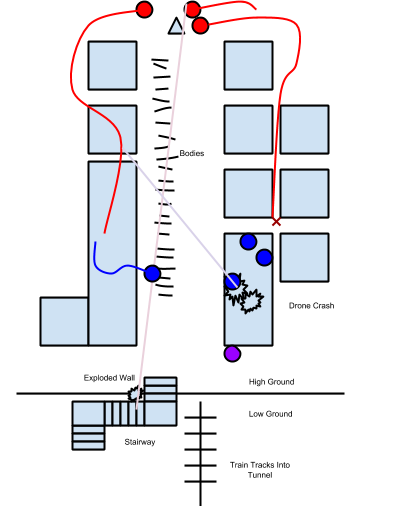
\includegraphics[width=8cm]{img/ch15_battle_map.png}
\footnote{\textbf{Suko T }Ooo a battle map!  Pretty sweet. \textsubscript{01/31/13 5:41pm}}\footnote{$\rightarrow$\textbf{Rebecca S. }I like how Lackovich is purple... suggesting half ``good team'', half ``bad team''.  Should we take this as foreshadowing? ;) \textsubscript{02/03/13 12:10am}}\footnote{$\rightarrow$\textbf{Nathaniel Ford }Ahahaha. No comment. \textsubscript{02/07/13 4:45pm}}\footnote{$\rightarrow$\textbf{Suko T }+1 \textsubscript{02/14/13 1:32am}}



\vspace{\fill}

\begin{flushright}
\textsubscript{last edited by \textbf{Suko T} @ 06/19/15 4:12pm}
% Exported @ 08/23/15 11:36pm
\end{flushright}

